\begin{frame}[fragile]{dimensions of arbitrary metric spaces}

\textbf{vector space dimension $(d)$}: what we're used to, only applies to $\mathbb{R}^d$
\vspace{0.05in}

\hspace{0.2in}...

\vspace{0.05in}
\textbf{Hausdorff dimension $(h)$}: the ``ideal'' generalization of dimensions to any metric space; can handle fractional dimensions, and is often associated with fractals
\begin{center}
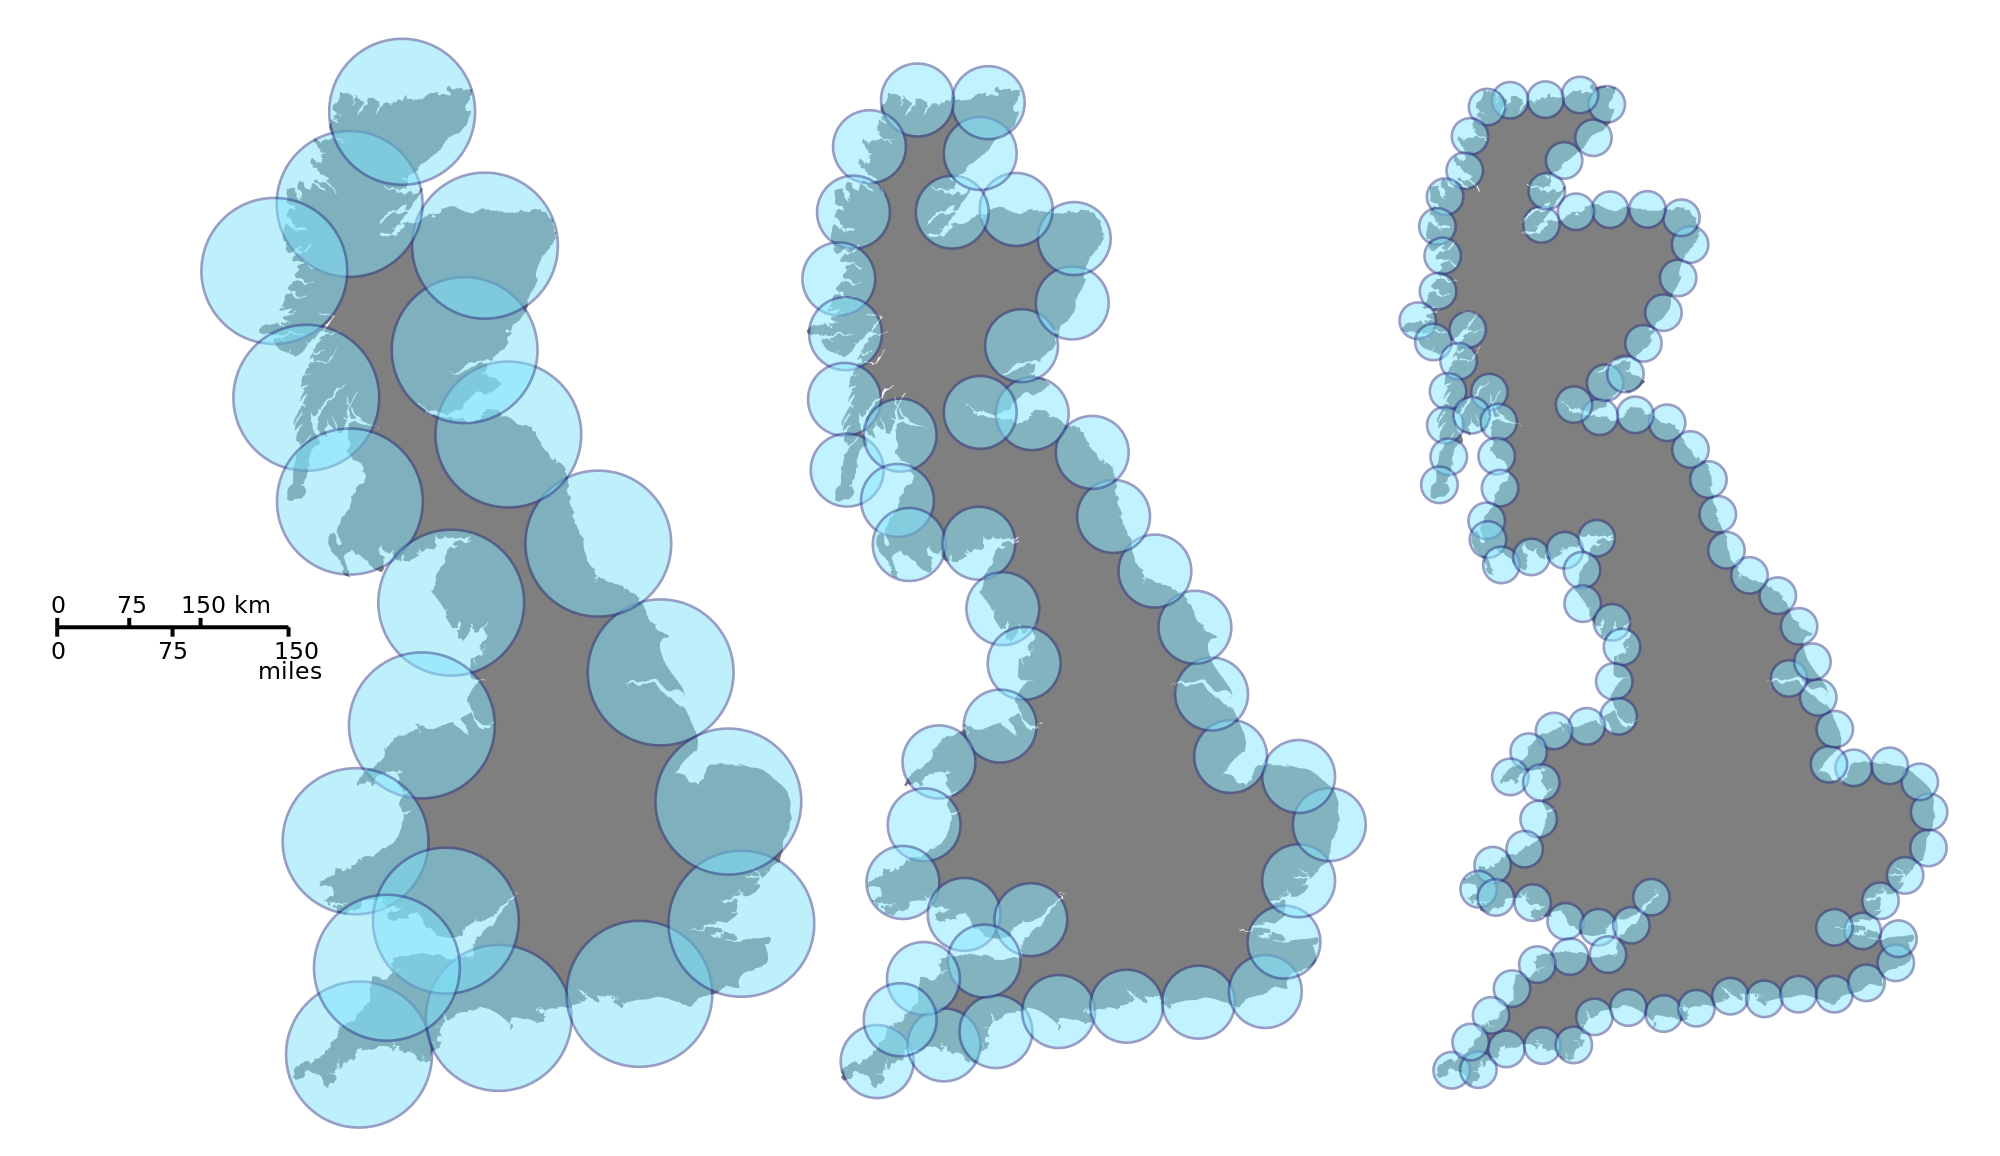
\includegraphics[width=6cm]{covertree/gb-hausdorff.png}
\end{center}

%dimension of the ``fractall'' coastline of Britain is about 1.25

\textbf{open problem}: create a data structure that lets us query nearest neighbors in time $O(h \log n)$; is it even possible?
\end{frame}

%%%%%%%%%%%%%%%%%%%%%%%%%%%%%%%%%%%%%%%%

\begin{frame}[fragile]{dimensions of arbitrary metric spaces}

Given a metric space $X$ with distance $d : X \times X \to \mathbb{R}$, define
\vspace{0.15in}

\textbf{ball of radius $r$ centered at point $p$ }:
$$
B(p,r) = \{q \in X : d(p,q) \le r \}
$$
%\vspace{0.15in}

%\textbf{expansion constant $(c)$}: the smallest value $c \ge 2$ such that
%$$
%|B(p,2r)| \le c|B(p,r)|
%$$
%for every $p$ in the metric space $X$ and $r\ge0$.

\textbf{expansion constant}:
$$
c = \sup_{p\in X, r\ge0} \left\{
    \frac{|B(p,2r)|}{|B(p,r)|}
      \right\}
$$

\hrule

\vspace{0.15in}
properties of the expansion constant:
\begin{enumerate}
\item dimension $(=\log c)$ of $\mathbb{R}^n$ is $O(n)$
\item roughly captures the ``intrinsic dimensionality'' of $X$
\item adding a single new point to $X$ can increase $c$ by an arbitrary amount;

there are subsets of $\mathbb{R}^2$ with $c=\infty$
\end{enumerate}

\end{frame}

%%%%%%%%%%%%%%%%%%%%%%%%%%%%%%%%%%%%%%%%

\begin{frame}[fragile]{data structures: bounds with arbitrary metric}

\begin{center}
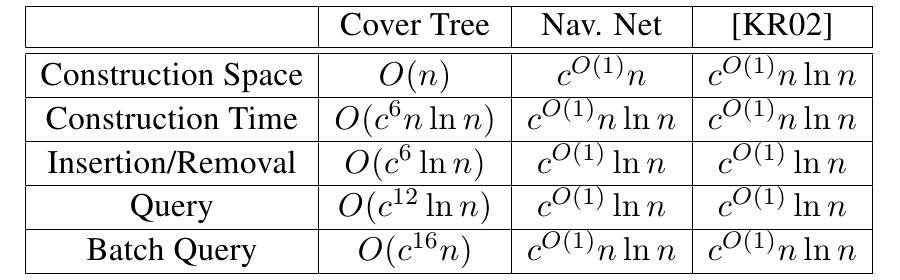
\includegraphics[width=12cm]{covertree/runtimes}
\end{center}

Karger and Ruhl, Symposium on the Theory of Computing, 2002

\vspace{0.15in}
Krauthgamer and Lee, Symposium on Discrete Algorithms, 2004

\vspace{0.15in}
Beygelzimer, Kakade, and Langford, ICML, 2006

\vspace{0.15in}
\textbf{open problem}: construct a data structure in time $O(c^{O(1)}n)$ for some dimensionality $c$; is it even possible?
\vspace{0.15in}

\end{frame}
